\documentclass[]{article}

\usepackage{graphicx}
\usepackage[spanish]{babel}
\usepackage[utf8]{inputenc}
\usepackage{hyperref}

%opening
\title{Reporte Anual 2019}
\author{Juan Irving Vásquez Gómez\\ Proyecto 1507}

\begin{document}
	
	\maketitle
	
	%\begin{abstract}
	
	%\end{abstract}
	
	\section{Información del proyecto}
	
	\begin{description}
		\item[Proyecto 1507:] Arquitecturas de sistemas embebidos para la investigación científica y la integración de tecnologías.
		\item[Propósito del proyecto] ``Consolidar  los  grupos  de  investigación  de  las  LGAC  del  IPN  CIDETEC,  a  través  de  la  investigación científica y la integración de tecnologías utilizando arquitecturas de sistemas embebidos. Proponer nuevos  nichos  de  investigación  y  desarrollos  tecnológicos  que  impacten  en  los  programas  de posgrado que se ofertan" \cite{proyecto1507}. 
		\item[Objetivo] ''Proponer el diseño, análisis e implementación de soluciones utilizando arquitecturas de sistemas embebidos, enfocándose en lo general a la ejecución intrínseca de algoritmos originales obtenidos 
		de  diferentes  investigaciones  y  bajo  vertientes  de  computación  inteligente,  cómputo  no convencional, robótica y visión artificial, entre otras. La investigación científica y la integración de tecnologías permitirán la consolidación de grupos de trabajo a través de la colaboración" \cite{proyecto1507}.
	\end{description}
	
	
\section{Resumen}

En este reporte se describen las actividades correspondientes al periodo comprendido entre septiembre de 2018 y agosto de 2019. Los principales resultados de este periodo se encuentren reflejados en los productos publicados. Tres artículos indexados en el JCR, un artículo en el índice CONACYT, un artículo en congreso internacional y dos artículos de divulgación. Dichas publicaciones han sido resultado del trabajo que se lleva con estudiantes de maestría, colaboración con investigadores de la institución receptora y colaboración con investigadores fuera de la institución receptora. Estos productos satisfacen el primer objetivo de investigación, \textit{``Analizar, diseñar e implementar algoritmos, aplicados a diferentes problemas de la computación inteligente, que se ejecuten de manera intrínseca en plataformas o arquitecturas de sistemas embebidos"}\cite{anexo2actualizado}.

Sobre el segundo objetivo de investigación, \textit{``Elaborar propuestas para proyectos de investigación y aplicar en las convocatorias respectivas (SIP, CONACYT, SECITI CDMX, etc.). Posteriormente se debe participar en el desarrollo del proyecto sometido y aceptado. También participará íntegramente en proyectos de investigación que desarrolle el grupo de trabajo"}\cite{anexo2actualizado}.  Se ha participado en los diversos proyectos del grupo de trabajo y se participó en la convocatoria de ciencia básica 2018. El resultado fue aprobado sujeto a presupuesto. Sin embargo no se obtuvo presupuesto. Actualmente se elabora una nueva propuesta para la convocatoria de Ciencia de frontera 2019.

Finalmente con respecto al objetivo de investigación tres, \textit{``Consolidación de grupos de trabajo a través de la colaboración"}\cite{anexo2actualizado}. Se mantiene la colaboración con el grupo de cómputo inteligente del CIDETEC y se ha comenzado a buscar universidades en el extrajero con las cuales entablar colaboración. 

En las siguientes secciones se detallan los productos obtenidos, la metodología seguida y las conclusiones.


\section{Actividades realizadas}
\label{sec:actividades}
	


Las actividades se han clasificado en tres tipos: Investigación, formación de recursos humanos y vinculación o divulgación de la ciencia.
	
\subsection{Investigación}
	
\input{../../productividad.tex}

\input{../../enviados.tex}

\subsection{Formación de recursos humanos}

Durante el periodo se graduó a dos estudiantes de maestría y se impartieron clases en el posgrado.

\input{../../formacion.tex} Se participó en diversos comités tutoriales.

\subsection{Vinculación o divulgación de la ciencia}

\begin{itemize} 
\item Rodriguez Hernandez, Erick and Vasquez-Gomez, JI, Enseñando a volar a un dron,\textit{ Komputer Sapiens,} (2019)
\end{itemize} 



\section{Metodología}

En este año se propusieron diversas actualizaciones al anexo 2 del proyecto, el cual describe en detalle las actividades del proyecto. Las modificaciones se encuentran en \cite{anexo2actualizado}. Dado que yo entré en sustitución del catedrático original, se decidió actualizar el anexo 2 tomando en cuenta mi primer año de trabajo (2016) como el año 1. De acuerdo a dicha actualización, se agregó el objetivo 3: ``Consolidación de grupos de trabajo a través de la colaboración", que se encuentra como parte del propósito del proyecto pero no estába reflejado en los objetivos. Además, se reajustaron las fechas de diversos productos esperados. El avance actual se resume en la figura \ref{fig:avances}. Como se puede observar en el calendario se ha cumplido con la parte de investigación (actividades 1.1 y 1.2) y se está trabajando en la elaboración de patentes (actividad 1.3) y registro de software. Sin embargo, debido a los largos procesos involucrados en el patentamiento y licenciamiento, no se ha concretado el registro de una patente. También es señalable que se están visualizando diversas formas de colaboración con grupos de trabajo en México y en extranjero (Actividad 3.1). Esperamos para el siguiente año, la realización de una estancia de investigación del catedrático. 


\section{Conclusiones}

Consideramos que durante este periodo se cumplieron los objetivos de producción científica y ésta va de acuerdo a la temática planteada en el proyecto. Se continuará participando en las diversas convocatorias de proyectos a fin de conseguir recursos para la investigación. Finalmente, se aumentarán esfuerzos en el licienciamiento y patentamiento de productos derivados.


\begin{figure}
	\centering
	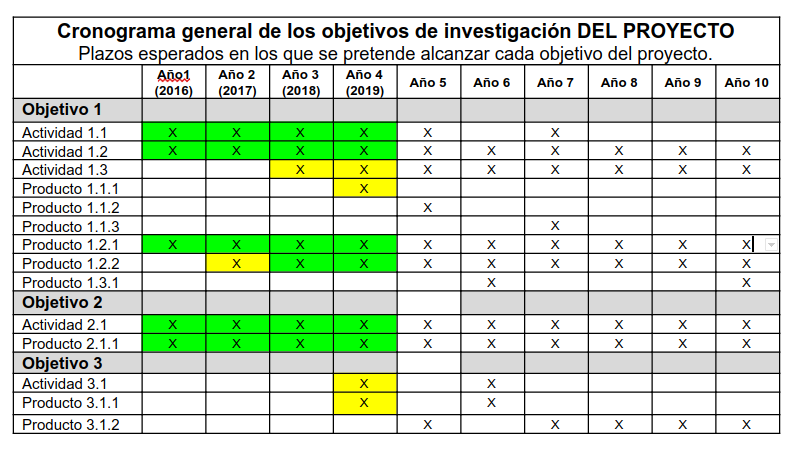
\includegraphics[width=\linewidth]{avances}
	\caption{}
	\label{fig:avances}
\end{figure}


\bibliographystyle{plain}
\bibliography{referencias}
	
\end{document}
